\section{Preliminary Results}\label{preliminary-results}

To preface, we have only begun exploratory data analysis following the
finalization of our analysis plan, updated with the feasibility review
from Professor Chiang. With the decision made to exclude the water
basins out of Great Britain, our training and test data will be drawn
from the following regions:

\begin{itemize}
\tightlist
\item
  \texttt{camels}, a database of 671 US water basins, of which 631
  contain sufficient data
\item
  \texttt{camelsaus}, a database of 561 Australian water basins, of
  which 541 contain sufficient data
\end{itemize}

Below is a map of the basins available in the two databases.

\begin{figure}
\centering
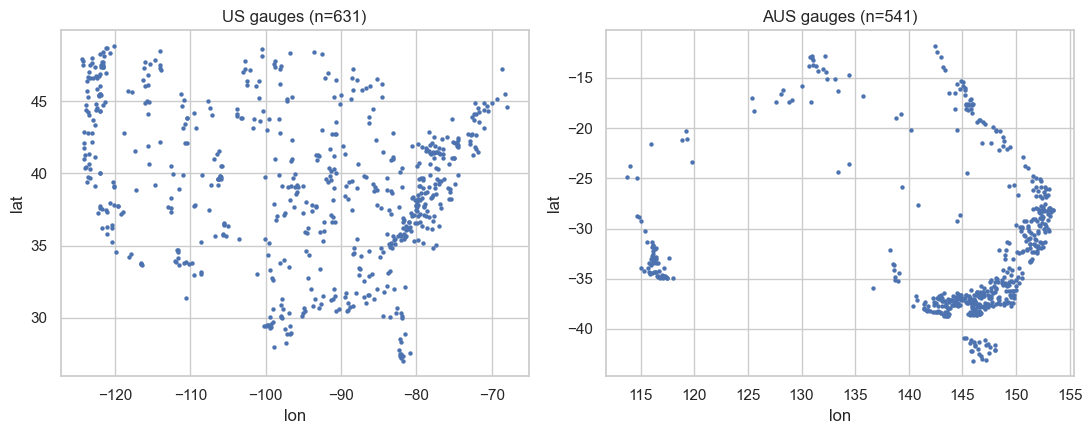
\includegraphics[width=1\linewidth,height=\textheight,keepaspectratio]{figures/basin-map.png}
\caption{Map of the basins available in the \texttt{camels} and
\texttt{camelsaus} databases.}\label{fig:basin-map}
\end{figure}

To arrive at the set of water basins with sufficient data we applied the
following thresholds:

\begin{itemize}
\tightlist
\item
  At least 15 years of valid water flow data.
\item
  At most 15\% of missing window days.
\end{itemize}

The following figures provide comparisons of the two databases.

\begin{figure}
\centering
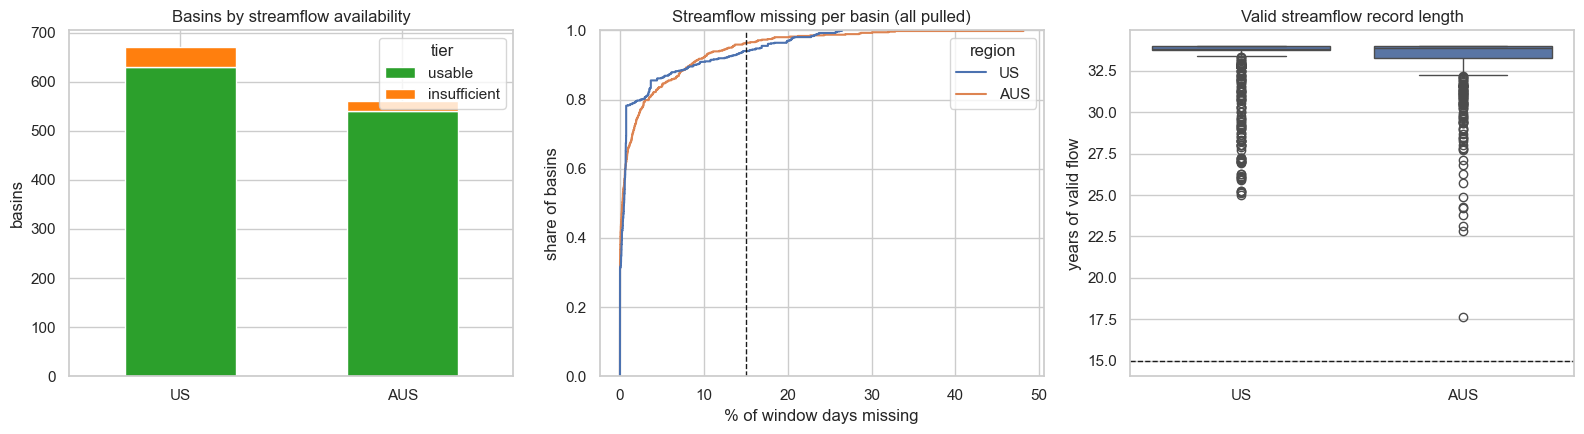
\includegraphics[width=1\linewidth,height=\textheight,keepaspectratio]{figures/region-comparison.png}
\caption{Comparison of the \texttt{camels} and \texttt{camelsaus}
databases.}\label{fig:region-comparison}
\end{figure}

Below we dril down into the availability of streamflow data over time,
from the early 1980s to the mid 2010s.

\begin{figure}
\centering
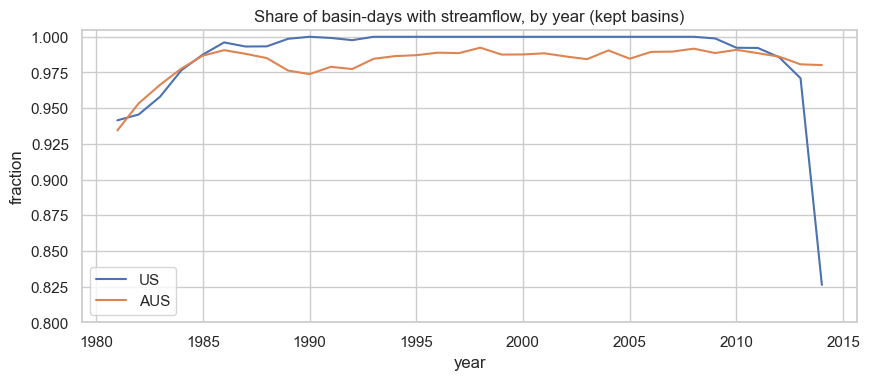
\includegraphics[width=1\linewidth,height=\textheight,keepaspectratio]{figures/missingness-by-year.png}
\caption{Availability of streamflow data by
year.}\label{fig:missingness-by-year}
\end{figure}

To get an idea of the data present for each basin, we zoom in below on a
single basin.

\begin{figure}
\centering
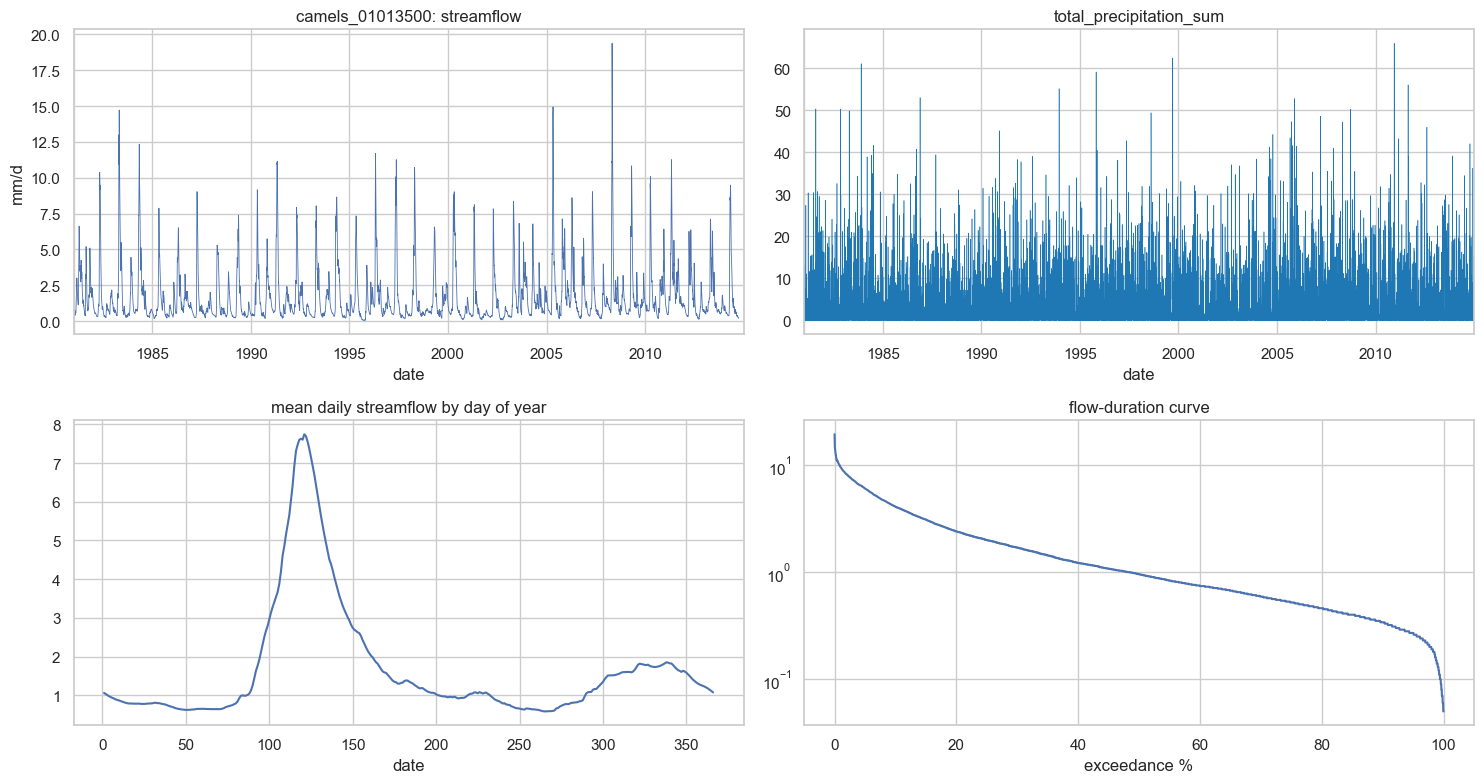
\includegraphics[width=1\linewidth,height=\textheight,keepaspectratio]{figures/example-basin.png}
\caption{Streamflow data for a single example
basin.}\label{fig:example-basin}
\end{figure}

Note the seasonal spikes \textasciitilde120 days into the year where
waterflow rises following spring precipitation. Our immediate next steps
are to define the temporal split of our training and test data, and the
locational blocking of our water basins, to inform k-fold validation.
